%
% chapter.tex
%
% (c) 2023 Prof Dr Andreas Müller
%
\chapter{Erste Variation
\label{buch:chapter:variation}}
\kopflinks{Erste Variation}
In Kapitel~\ref{buch:chapter:fuvar} wurde gezeigt, wie Extremalprobleme
für Funktionen mehrerer Variablen mit Hilfe der Richtungsableitung
gelöst werden können.
Die Unbekannte war ein Vektor in einem endlichdimensionalen $\mathbb{R}^n$.
Die Variationsrechnung verallgemeinert die Fragestellung auf das Problem,
eine Funktion zu finden, die eine von der Funktion abhängige Grösse
minimiert.
Die Menge der Funktion bilden wie die Vektoren in $\mathbb{R}^n$
einen Vektorraum, der aber keine endliche Basis mehr hat.
Die Idee der partiellen Ableitung nach ``Basisrichtungen'' ist
damit nicht mehr anwendbar, es muss ein alternativer Ansatz gefunden
werden.
Es wird sich zeigen, dass die Idee der Richtungsableitung anwendbar
bleibt.
Wie im endlichdimensionalen Fall entsteht eine Bedingung, die sich
mit dem Skalarprodukt formulieren lässt.
Das Fundamentallemma in
Abschnitt~\ref{buch:variation:section:fundamentallemma}
schliesst dann aus dem Verschwinden aller Richtungsableitungen 
auf das Verschwinden einer Funktion, was auf die
Euler-Lagrange-Differentialgleichung und damit auf eine allgemeine
Methode zur Lösung von Variationsproblemen führt.

%
% 1-problem.tex
%
% (c) 2023 Prof Dr Andreas Müller
%
\section{Problemstellung
\label{buch:variation:section:problemstellung}}
\kopfrechts{Problemstellung}
Das Brachistochronenproblem, welches Johann Bernoulli im Jahr 1696
gestellt hat, war nicht das erste Optimierungsproblem für eine 
gesuchte Funktion, welches Physiker betrachtet haben.
Aber es darf als Ausgangspunkt für die Entwicklung der Variationsrechnung
betrachtet werden.
Alle diese Probleme zeichnen sich dadurch aus, dass Extremwerte
einer Grösse, die von allen Werten einer unbekannten Funktion abhängt,
gefunden werden sollen.
Die von Euler und Lagrange entwickelte Theorie zeigt, dass eine
Lösung für diese globale Eigenschaft immer auf eine lokale Bedingungen,
genauer auf eine Differentialgleichung reduziert werden kann, für deren
Lösung bereits eine ausgefeilte Theorie existiert.

%
% Der Anfang: das Brachistochronenproblem von Bernoulli
%
\subsection{Der Anfang: Das Brachistochronenproblem von Bernoulli
\label{buch:variation:problem:subsection:brachistochrone}}
%
% brachistochronenproblem.tex -- Brachistochronenproblem
%
% (c) 2021 Prof Dr Andreas Müller, OST Ostschweizer Fachhochschule
%
\documentclass[tikz]{standalone}
\usepackage{amsmath}
\usepackage{times}
\usepackage{txfonts}
\usepackage{pgfplots}
\usepackage{csvsimple}
\usetikzlibrary{arrows,intersections,math}
\begin{document}
\def\skala{1}
\def\r{1.5}
\pgfmathparse{3.14159/180}
\xdef\m{\pgfmathresult}
\def\xwert#1{\r*((#1)*\m-sin(#1))}
\def\ywert#1{\r*(cos(#1)-1)}
\def\punkt#1{ ({\r*((#1)*\m-sin(#1))},{\r*(cos(#1)-1)}) }
\begin{tikzpicture}[>=latex,thick,scale=\skala]

\draw[color=gray!50] plot[domain=0:360,samples=360]
	({\r*((\x)*\m-sin(\x))},{\r*(cos(\x)-1)});

\draw[->] (-0.1,0) -- (10,0) coordinate[label={$x$}];
\draw[->] (0,0.1) -- (0,-3.5) coordinate[label={left:$y$}];

\draw ({\m*\r*180},0.05) -- ({\m*\r*180},-0.05);
\node at ({\m*\r*180},0) [above] {$\frac{\pi}2\mathstrut$};
\draw ({\m*\r*360},0.05) -- ({\m*\r*360},-0.05);
\node at ({\m*\r*360},0) [above] {$\pi\mathstrut$};

\draw[line width=0.2pt]  ({\xwert{60}},0) -- \punkt{60};
\node at ({\xwert{60}},0) [above] {$a\mathstrut$};
\draw ({\xwert{60}},0.05) -- ({\xwert{60}},-0.05);

\draw[line width=0.2pt]  ({\xwert{160}},0) -- \punkt{160};
\node at ({\xwert{160}},0) [above] {$b\mathstrut$};
\draw ({\xwert{160}},0.05) -- ({\xwert{160}},-0.05);

\draw[color=red,line width=1.2pt] plot[domain=60:160,samples=100]
	({\r*((\x)*\m-sin(\x))},{\r*(cos(\x)-1)});

\fill[color=red] \punkt{60} circle[radius=0.08];
\node at \punkt{60} [above right] {$A$};
\fill[color=red] \punkt{160} circle[radius=0.08];
\node at \punkt{160} [below] {$B$};
\fill[color=red] \punkt{100} circle[radius=0.08];
\node at \punkt{100} [below left] {$M$};

\end{tikzpicture}
\end{document}


Im Jahr 1696 publiziert der Basler Mathematiker Johann Bernoulli, damals
Professor für Mathematik in Groningen das folgende Problem in der
von Leibniz herausgegebenen Zeitschrift {\em Acta eruditorum}:
\begin{center}
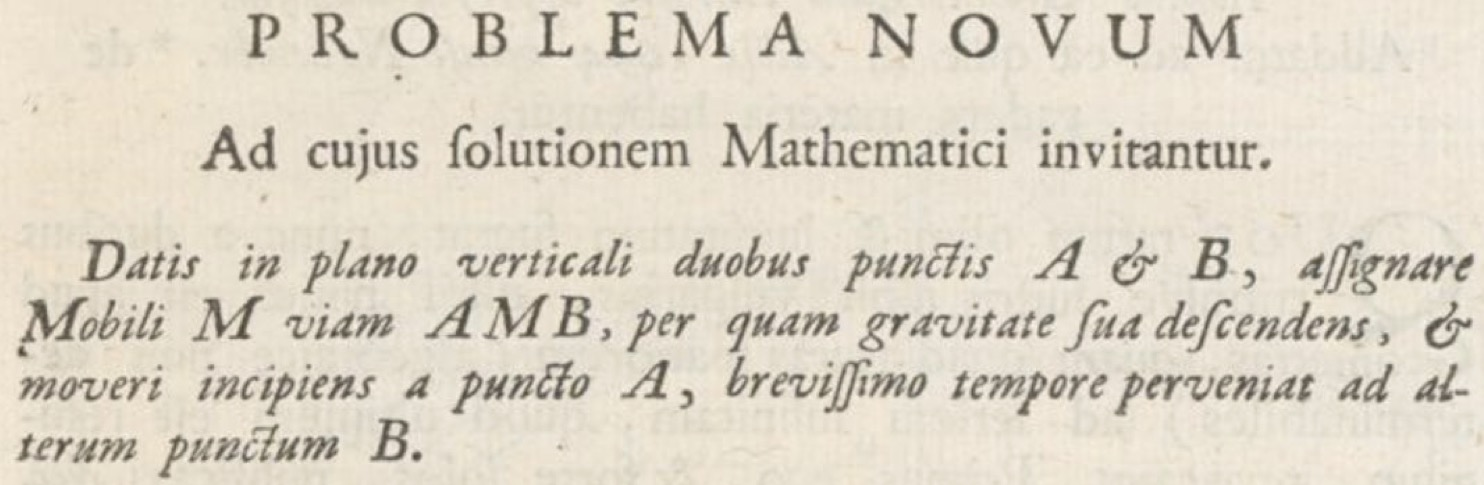
\includegraphics[width=0.8\textwidth]{chapters/020-variation/images/latein.jpg}
\end{center}
Zu deutsch:
\begin{quote}
Neue Aufgabe, zu deren Lösung die Mathematiker eingeladen werden.
Gegeben zwei Punkte $A$ und $B$ in einer vertikalen Ebene, finde
die Bahn $AMB$ eines Punktes $M$, der unter der Wirkung seines
Gewichtes in kürzester Zeit vom Punkt $A$ zum anderen Punkt $B$ absteigt.
\end{quote}
Die Situation der Aufgabenstellung ist in
Abbildung~\ref{buch:variation:fig:brachistochronenproblem}
dargestellt.
Bernoulli hat als Lösung gefunden, dass die Kurve eine Ausschnitt
aus einer Zykloide (in der Abbildung grau) sein muss.
Seine Lösung beruhte auf der Beobachtung, dass sich das Problem analog
zu einem Lichtausbreitungsproblem ist, für welches Fermat bereits
eine Lösung gefunden hat.

Da die Reibung vernachlässigt wird, ist die Energie des Massepunktes
erhalten.
Sie setzt sich aus der potenziellen und der kinetischen Energie
zusammen.
Die potenzielle Energie ist $-mgy$, die kinetische Energie ist
$\frac12mv^2$.
Die Energieerhaltung wird daher zu
\[
E=\frac12mv^2-mgy
\qquad\Rightarrow\qquad
v
=
\sqrt{2g}\!\sqrt{\frac{E}{gm}+y}
=
\!\sqrt{2(C+y)}.
\]
Durch Wahl einer anderen Zeiteinheit kann die Gleichung noch weiter
vereinfacht zu
\(
v = \sqrt{C+y}
\)
vereinfacht werden.
Gesucht ist also die zeitlich kürzeste Bahn eines Teilchens, 
dessen Geschwindigkeit auf bekannte Art $v(y)$ von der vertikalen
Koordinate abhängt.

%
% Das Fermat-Problem
%
\subsection{Das Fermat-Prinzip}
Bereits Fermat hat erkannt, dass das Brechnungsgesetz von Snellius
als Lösung eines Extremalproblems verstanden werden kann.

\begin{satz}[Fermat]
Sie $c/n_i$ die Geschwindigkeit, mit der sich Licht im Medium $M_i$
ausbreitet.
Ein Lichtstrahl von $A_1$ nach $A_2$ geht durch denjenigen Punkt $B$ 
auf der Grenzfläche zwischen den Medien, für den sich die Sinus der
Winkel $\alpha_i$ zwischen den Strahlen und der Normalen zur Grenzfläche
umgekehrt wie die $n_i$ verhalten, wenn also das Brechungsgesetz
\[
\frac{\sin\alpha_1}{\sin\alpha_2}
=
\frac{n_2}{n_1}
\]
gilt.
\end{satz}

\begin{proof}
Ohne der Beschränkung der Allgmeinheit können wir auf die Betrachtung
einer Ebene beschränken, die die beiden Punkte $A_i$ enthält und senkrecht
auf der Grenzfläche steht.
Wir dürfen weiter annehmen, dass die $x$-Achse in der Grenzfläche liegt 
und die Punkte $A_i$ die Koordinaten $(x_i,y_i)$ und der Punkt $B$ die
Koordinaten $(x,0)$ hat.
Es ist derjenige Punkt $x$ zu bestimmen, für den die Lichtzeit entlang 
des Pfades $A_1BA_2$ minimal wird.
Diese Zeit ist
\begin{align*}
t
&=
\frac{\overline{A_1B}}{c/n_1}
+
\frac{\overline{BA_2}}{c/n_2}
\\
ct
&=
n_1\overline{A_1B}
+
n_2\overline{A_2B}
\\
&=
n_1\!\sqrt{(x-x_1)^2 + y_1^2}
+
n_2\!\sqrt{(x_2-x)^2 + y_2^2}
\end{align*}
Das Minimum wird bei einer Nullstelle der Ableitung nach $x$ gefunden,
also bei einer Lösung der Gleichung
\begin{align*}
0
&=
n_1\frac{2(x_1-x)x}{\sqrt{(x_1-x)^2+y_1^2}}
+
n_2\frac{-2(x-x_2)x}{\sqrt{(x_2-x)^2+y_2^2}}.
\intertext{Indem man den zweiten Term auf der rechten Seite auf die linke
Seite bringt und durch $x$ dividiert, erhält man}
n_1
\frac{x_1-x}{\sqrt{(x_1-x)^2+y_1^2}}
&=
n_2
\frac{x-x_2}{\sqrt{(x_2-x)^2+y_2^2}}.
\end{align*}
Der Nenner ist auf beiden Seiten die Hypothenuse eines rechtwinkligen
Dreiecks, welches als Ankathete die Normale zur Grenzfläche hat.
Der Zähler ist die Gegenkathete des Winkels $\alpha_i$ zwischen der
Hypothenuse und der Normalen.
Daher ist der Quotient der Sinus des Winkels oder
\begin{equation}
n_1 \sin\alpha_1 = n_2 \sin\alpha_2.
\label{buch:variation:problem:eqn:snelliusinvariante}
\end{equation}
Die Gleichung~\eqref{buch:variation:problem:eqn:snelliusinvariante}
ist gleichbedeutend mit dem Brechungsgesetz
\[
\frac{\sin\alpha_1}{\sin\alpha_2}
=
\frac{n_2}{n_1}
\]
von Snellius.
\end{proof}

Der Satz von Fermat etabliert das Brechungsgsetz also Lösung eines
Extremalproblems.
Die Natur wählt für einen Lichtstrahl den zeitlich kürzesten Weg.
Der Beweis des Satzes von Fermat zeigt, dass entlang des Lichtstrahls
an jeder Grenzfläche zwischen Medien die Bedingung
\eqref{buch:variation:problem:eqn:snelliusinvariante}
erfüllt.
Wenn die optische Dichte $n$ eine Funktion von $n(y)$ ist, dann
wird der Lichtstrahl nicht nur in diskreten Punkten geknickt, sondern
entlang des ganzen Strahles gekrümmt.
Folgt der Strahl der Kurve $x(y)$, die mit der vertikalen den Winkel
$x'(y) = \tan\alpha(y)$ einschliesst.
Damit lässt sich auch die Sinus-Funktion ausdrücken, es gilt
\[
\sin\alpha(y)
=
\frac{x'(y)}{\pm\!\sqrt{x'(y)^2+1}}.
\]
Aus der Form~\eqref{buch:variation:problem:eqn:snelliusinvariante}
des Brechungsgesetztes wird dann die Gleichung
\begin{equation}
n_1\sin\alpha(y)
=
\frac{n_1(y)x'(y)}{\pm\!\sqrt{x'(y)^2+1}}
=
\operatorname{const}
\qquad\Rightarrow\qquad
\frac{n_1(y)^2x'(y)^2}{x'(y)^2+1}=C.
\label{buch:variation:eqn:fermatdgl}
\end{equation}
Dies ist eine Differentialgleichung für die Funktion $x(y)$.
Sie kann auch in die Form
\[
x'(y)^2
=
\frac{C}{(n_1(y)^2-C)}
\]
gebracht werden.

%
% Das Brachistochronenproblem als Lichtausbreitungsproblem
%
\subsubsection{Das Brachistochronenproblem als Lichtausbreitungsproblem}
Das Fermat-Prinzip besagt, dass ein Lichtstrahl, der sich in einem Medium
mit der Geschwindigkeit $c/n(y)$ ausbreitet, die Gleichung 
\eqref{buch:variation:eqn:fermatdgl} erfüllt.
Beim Brachistochronenproblem ist die Geschwindigkeit $v(y)=\!\sqrt{C-y}$ und 
damit $n(y) = c/\!\sqrt{C-y}$.
Eine Brachistochrone ist also eine Kurve, die die aus
\eqref{buch:variation:eqn:fermatdgl} folgende Gleichung
\begin{equation}
\frac{x'(y)^2}{(1+x'(y)^2)(C-y)} = K
\label{buch:variation:problem:eqn:bernoullidgl}
\end{equation}
erfüllen.

%
% Die Bernoullische Lösung
%
\subsubsection{Die Bernoullische Lösung}
Bernoulli hat gefunden, dass die Brachistochrone ein Zykloidenbogen ist.
Dies lässt sich dadurch verifizieren, dass man die Parametrisierung
einer Zykloide in die
Gleichung~\eqref{buch:variation:problem:eqn:bernoullidgl}
einsetzt.
Die Zykloide hat die Parametrisierung
\[
\left.
\begin{aligned}
x &= r(\varphi - \sin\varphi) 
\\
y &= r(1-\cos\varphi)
\end{aligned}
\right\}
\quad
\text{mit der Ableitung}
\quad
\left\{
\begin{aligned}
\dot{x}(\varphi) &= r(1-\cos\varphi)\\
\dot{y}(\varphi) &= r\sin\varphi
\end{aligned}
\right.
\]
für $\varphi\in\mathbb{R}$.
Die Ableitung ist
\[
x'(y)
=
\frac{\dot{x}(\varphi)}{\dot{y}(\varphi)}
=
\frac{1-\cos\varphi}{\sin\varphi}.
\]
Eingesetzt in \eqref{buch:variation:problem:eqn:bernoullidgl}
wird daraus
\[
\frac{\dot{x}(\varphi)^2}{
(\dot{y}(\varphi)^2 +\dot{x}(\varphi)^2)
(C-r(1-\cos\varphi))
}
=
\frac{(1-\cos\varphi)^2}{
((1-\cos\varphi)^2+\sin^2\varphi)
(C-r+r\cos\varphi)
}
=
K.
\]
Ausmultiplizieren im Nenner ergibt
\[
\frac{(1-\cos\varphi)^2}{
(1-2\cos\varphi+\cos^2\varphi+\sin^2\varphi)
(C-r+r\cos\varphi)
}
=
\frac{1-\cos\varphi}{
2(C-r+r\cos\varphi)
}
\]

%
% Das Brachistochronenproblem als Variationsproblem
%
\subsection{Das Brachistochronenproblem als Variationsproblem
\label{buch:variation:problem:subsection:variationsproblem}}
Die Bernoullische Lösung des Brachistochronenproblems verwendet die
Analogie zum Fermat-Prinzip.
Eine solche Analogie ist nur selten möglich, daher soll das Problem
jetzt in eine Form gebracht werden, in die auch viele ähnliche
Optimierungsproblem gebracht werden können.

Wir erinnern daran, dass die Geschwindigkeit des Massepunktes durch
$v(y)=\sqrt{C-y}$ gegeben ist.
Damit lässt sich die Zeit berechnen, die der Massepunkt entlang der
Lösungskurve braucht, wenn man diese als Funktion $y(x)$ mit beschreibt.
Die Punkte $A$ und $B$ sollen die $x$-Koordinaten $a$ bzw.~$b$ haben.
Für das Kurvenstück zwischen den $x$-Koordinaten $x$ und $x+\Delta x$
braucht der Massepunkt die Zeit
\[
\frac{ \sqrt{\Delta x^2 + \Delta y^2} }{v(y)}
=
\frac{ \sqrt{1 + y'(x)^2} }{ v(y) } \Delta x.
\]
Die Zeit ist das Integral
\begin{equation}
t
=
\int_a^b \frac{\sqrt{1+y'(x)^2}}{v(y(x))}\,dx
=
\int_a^b \sqrt{\frac{1+y'(x)^2}{C-y(x)}}\,dx.
\label{buch:variation:problem:eqn:brachint}
\end{equation}
Der Integrand auf der rechten Seite hängt nur von den Funktion $y(x)$
und $y'(x)$ ab.
Dies kommt vor allem daher, dass die Geschwindigkeit nur von $y$ abhängt,
nicht auch noch von $x$.
Im Allgemeinen wird man also davon ausgehen müssen, dass der Integrand
auch noch von $x$ abhängt.
Die Variationsrechnung befasst sich mit Problemen, in denen Funktionen
gefunden werden müssen, die ein Integral wie das in
\eqref{buch:variation:problem:eqn:brachint}
minimiert oder maximiert werden müssen.

\begin{definition}[Lagrange-Funktion des Brachistochronenproblems]
Die Lagrange-Funk\-tion des Brachistochronenproblems ist der
Integrand des Integrals
\eqref{buch:variation:problem:eqn:brachint},
\index{Lagrange-Funktion}%
also die Funktion
\[
L(x,y,y')
=
\sqrt{\frac{1+y^{\prime 2}}{C-y}}.
\]
\end{definition}

%
% Funktionale
%
\subsection{Funktionale
\label{buch:variation:problem:subsection:funktionale}}
Die Variationsrechnung löst Optimierungsproblem, die von einer
Funktion abhängen.
Um dies mathematisch präzis zu fassen, ist zunächst nötig, die Menge
der in Frage kommenden Funktionen so einzuschränken, dass die interessierende
Grösse überhaupt wohldefiniert ist.

%
% Vektorräume
%
\subsubsection{Vektorräume}
Zunächst sind die gemeinsamen algebraischen Eigenschaften zu charakterisieren,
die wir von den für unsere Untersuchungen zweckmässigen Funktionenmengen
erwarten.

\begin{definition}[Vektorraum]
Ein Vektorraum über den reellen Zahlen $\mathbb{R}$ ist einem Menge $V$ mit
zwei Operationen, der Addition und der Multiplikation mit Skalaren
\begin{align*}
    +\colon V\times V         &\to V : (u,v)\mapsto u+v
&
\cdot\colon \mathbb{R}\times V&\to V : (\lambda,v) \mapsto\lambda v
\end{align*}
mit den folgenden Eigenschaften.
\begin{enumerate}
\item
Es gelten die Assoziativgesetze
\begin{align*}
(u+v)+w&=u+(v+w)&&\text{für alle $u,v,w\in V$}\\
(\lambda \mu)v&=\lambda(\mu v)&&\text{für alle $\lambda,\mu\in\mathbb{R},\;v\in V$.}
\end{align*}
\item
Es gibt einen Vektor $0\in V$ mit der Eigenschaft $0+v=v$ für alle
Vektoren $v\in V$.
\item
Zu jedem Vektor $v\in V$ gibt es den entgegengesetzten Vektor $-v\in V$
mit der Eigenschaft, dass $-v+v=0$ ist.
\item
Die Addition von Vektoren ist kommutativ: $u+v=v+u$ für alle $u,v\in V$.
\item
Es gelten die Distributivgesetze 
\begin{align*}
(\lambda + \mu) v &= \lambda v + \mu v
	&\quad\text{für alle $\lambda,\mu\in\mathbb{R},\;v\in V$}\\
\lambda(u+v)      &= \lambda u + \lambda v
	&\quad\text{für alle $\lambda\in\mathbb{R},\;u,v\in V$}
\end{align*}
\end{enumerate}
\end{definition}

Die Mengen $\mathbb{R}^n$ erfüllen die genannten Eigenschaften, sind
also Vektorräume.
Die Definition eines Vektorraums ist aber viel allgemeiner, insbesondere
gehören dazu auch Mengen von Funktionen.
Damit wird es möglich, die Berechnungen in $\mathbb{R}^n$ auf Funktionen
auszudehnen.
Zum Beispiel bilden die stetigen Funktionen auf einem Intervall einen
Vektorraum, wie das folgende Beispiel zeigt.

\begin{beispiel}
Die Menge
\[
C([a,b])
=
\{f\colon[a,b]\to\mathbb{R}\mid \text{$f$ ist stetig}\}
\]
der stetigen Funktionen bildet einen Vektorraum.
Die Operationen sind die punktweise Addition von Funktionen und die
Multiplikation der Werte mit Skalaren, für $f,g\in C([a,b])$ und
$\lambda\in \mathbb{R}$ ist
\begin{align*}
(f+g)(x) &= f(x)+g(x)
&&\text{und}&
(\lambda f)(x) &= \lambda f(x).
\end{align*}
Entscheidend ist, dass die Addition von Funktionen und die Multiplikation
mit Skalaren nicht aus der Menge herausführt.
Tatsächlich wird in der Analysis gezeigt, dass die Summe stetiger Funktionen
wieder stetig ist und dass die Funktion $x\mapsto \lambda f(x)$ stetig,
wenn $f$ stetig ist.
Die übrigen Eigenschaften sind ebenfalls erfüllt, da sie bereits für die
Funktionswerte erfüllt sind.
\end{beispiel}

%
% Norm und Grenzwerte
%
\subsubsection{Norm und Grenzwerte}
Um Analysis zu betreiben, muss man ausdrücken können, dass eine Folge
von Funktionen konvergiert.
Dazu ist ein Abstandsbegriff zwischen Funktionen nötig.

\begin{definition}[Norm, normierter Raum]
Eine {\em Norm} auf einem Vektorraum $V$ ist eine Abbildung
\index{Norm}%
$\|\cdot\|\colon V\to\mathbb{R}^+_0$ mit nichtnegativen reellen Werten
und den folgenden Eigenschaften
\begin{itemize}
\item Definitheit: $\|v\|\ge 0$ für $v\in V$ mit Gleichheit 
genau dann, wenn $v=0$.
\index{Definitheit}%
\item Absolute Homogenität: Für alle Vektoren $v\in V$ und
\index{Homogenität}%
$\lambda\in\mathbb{R}$ gilt $\|\lambda v\| = |\lambda|\, \|v\|$.
\item Dreiecksungleichung: für alle Vektoren $u,v\in V$ gilt
\index{Dreiecksungleichung}%
$\|u+v\|\le \|u\|+\|v\|$.
\end{itemize}
Ein {\em normierter Raum} ist ein Vektorraum mit einer Norm.
\index{normierter Raum}%
\end{definition}

\begin{beispiel}
Der Vektorraum der stetigen Funktionen kann mit der Supremum-Norm
\[
\|f\| = \sup_{x\in[a,b]} |f(x)|
\]
zu einem normierten Raum gemacht werden.
Die Definitheit ist durch die Definition offensichtlich sichersgtellt.
Für $\|\lambda f\|$ finden wir
\[
\|\lambda f\|
=
\sup_{x\in[a,b]} |\lambda f(x)|
=
|\lambda|\,
\sup_{x\in[a,b]} |f(x)|
=
|\lambda|\, \|f\|,
\]
was die Homogenität zeigt.
Die Dreiecksungleichung folgt aus
\begin{align*}
\|f+g\|
&=
\sup_{x\in[a,b]} |f(x)+g(x)|
\\
&\le
\sup_{x\in[a,b]} (|f(x)|+|g(x)|)
\\
&\le
\sup_{x\in[a,b], y\in[a,b]} (|f(x)|+|g(y)|)
\\
&=
\sup_{x\in[a,b]} |f(x)|
+
\sup_{y\in[a,b]} |g(y)|
=
\|f\| + \|g\|.
\qedhere
\end{align*}
\end{beispiel}

Mit einer Norm ist es jetzt möglich, die Konvergenz von Folgen und den
Begriff des Grenzwertes zu definieren.

\begin{definition}[Cauchy-Folge, Grenzwert]
Eine Folge $(x_n)_{n\in\mathbb{N}}$ in $V$ in einem normierten Raum $V$
mit der Norm $\|\cdot\|$
heisst eine Cauchy-Folge, wenn es für jedes $\varepsilon>0$ eine
\index{Cauchy-Folge}%
$N\in \mathbb{N}$ gibt derart, dass
\[
\| x_n - x_m \| < \varepsilon
\quad\forall n,m\ge N.
\]
Der Vektor $x\in V$ heisst {\em Grenzwert} der Folge $(x_n)_{n\in\mathbb{N}}$,
\index{Grenzwert}%
wenn es zu jedem $\varepsilon > 0$ ein $N\mathbb{N}$ gibt derart, dass
\[
\|x_n-x\| < \varepsilon 
\quad\forall n\ge N.
\]
Die Folge $(x_n)_{n\in\mathbb{N}}$  in $V$ heisst {\em konvergent}, wenn
\index{konvergent}%
$x$ der Grenzwert von $(x_n)_{n\in\mathbb{N}}$ ist.
\end{definition}

Der durch die Supremum-Norm definierte Konvergenzbegriff ist die gleichmässige
Konvergenz.
Zur Erinnerung:
Eine Folge $f_n$ von Funktionen heisst gleichmässig konvergent gegen die
Funktion $f$, wenn es zu jedem
$\varepsilon >0$ ein $N\in\mathbb{N}$ gibt derart, dass
\[
|f_n(x) - f(x)|<\varepsilon\quad\forall n>N\text{ und }x\in [a,b].
\]
Die Supremum-Norm ist
\[
\|f_n(x) - f(x)\|
=
\sup_{x\in[a,b]} |f_n(x)-f(x)| < \varepsilon
\]
für alle $n>N$.
Dies ist genau die Konvergenz in der Norm $\|\cdot\|$.
Aus der Analysis ist bekannt, dass eine gleichmässig konvergente 
Funktionenfolge gegen eine stetige Funktion konvergiert.

\begin{definition}[Banach-Raum]
Ein normierter Raum $V$ heisst ein {\em Banach-Raum},
\index{Banach-Raum}%
wenn jede Cauchy-Folge in $V$ einen Grenzwert hat.
\end{definition}

\begin{beispiel}
Die Menge $C^1([0,2])$
der stetigen Funktionen auf dem Intervall $[0,2]$ ist ein normierter
Raum mit der Norm
\[
\|f\|_1
=
\int_0^2 |f(x)|\,dx,
\]
die auch die $L^1$-Norm heisst.
\index{L1-Norm@$L^1$-Norm}%
Zunächst ist nachzuprüfen, dass dies tatsächlich eine Norm ist.
Die Definitheit und die Homogenität von $\|\cdot\|_1$ ist klar, nur
die Dreiecksungleichung erfordert etwas Arbeit.
Für Funktionen $f,g\in L^1([0,2])$ gilt
\begin{align*}
\|f+g\|_1
&=
\int_0^2 |f(x)+g(x)|\,dx
\\
&\le 
\int_0^2 |f(x)|+|g(x)|\,dx
=
\int_0^2 |f(x)|\,dx
+
\int_0^2 |g(x)|\,dx
=
\|f\|_1+\|g\|_1,
\end{align*}
was die Dreeicksungleichung beweist.

Eine Cauchy-Folge in der $L^1$-Norm muss aber nicht unbedingt einen
stetigen Grenzwert haben.
Die Funktionen
\(
f_n(x) =
\begin{cases}
x^n&\quad x< 1\\
1&\quad x\ge 1
\end{cases}
\)
haben die $L^1$-Norm
\begin{align*}
\|f_n-f_m\|_1
=
\int_0^2 |f_n(x)-f_m|\,dx
\\
&=
\biggl|\int_0^1 x^n-x^m\,dx\biggr|
=
\biggl[
\biggl|
\frac{1}{n+1}x^{n+1}
-
\frac{1}{m+1}x^{m+1}
\biggr|
\biggr]_0^1
\\
&=
\biggl|
\frac{1}{n+1}
-
\frac{1}{m+1}\biggr|.
\end{align*}
Wegen
\[
\|f_n-f_m\|_1
<\varepsilon
\]
für $n,m>2/\varepsilon$ ist $f_n$ eine Cauchy-Folge in $L^1$.
In $L^1$ konvergiert die Folge $f_n$ gegen die Funktion
\[
f(x)
=
\begin{cases}
0&\quad x< 1\\
1&\quad x\ge 1.
\end{cases}
\]
Diese Funktion ist aber nicht stetig, da sie bei $x=1$ einen
Sprung hat.
Bezüglich der $L^1$-Norm ist $C^1([a,b])$ als im Allgemeinen
kein Banach-Raum.
\end{beispiel}

%
% Stetige und differenzierbare Funktionen
%
\subsubsection{Stetige und differenzierbare Funktionen}
Mit der Norm lässt sich auch die Stetigkeit von Abbildungen zwischen
normierten Räumen definieren.

\begin{definition}[Stetigkeit]
Eine Funktion $f\colon U\to V$ zwischen normierten Räumen heisst
{\em stetig im Punkt} $x\in U$, wenn es zu jedem $\varepsilon > 0$
\index{stetig in einem Punkt}%
ein $\delta > 0$
gibt derart, dass
\(
\|f(x)-f(y)\| < \delta
\)
wenn
\(
\|x-y\|<\varepsilon
\).
Eine Funktion $f\colon U\to V$ heisst {\em stetig}, wenn sie in
jedem Punkt von $U$ stetig ist.
\end{definition}

Das Bild einer Folge $x_n\in U$, die gegen $x_0\in U$ konvergiert,
ist eine Folge $f(x_n)$ in $V$.
Man sagt, $y\in V$ sei der Grenzwert von $f(x)$ für $x\to x_0$,
wenn $f(x_n)$ für jede solche Folge $x_n$ gegen $y$ konvergiert.
Der Grenzwert wird auch
\[
\lim_{x\to x_0} f(x)
=
y
\]
geschrieben.
Stetige Funktionen zeichnen sich wie in der Analysis der Funktionen
einer Variablen dadurch aus, dass der Grenzwert der Werte der Funktion
auf einer konvergenten Folge mit dem Funktionswert des Grenzwertes
übereinstimmt.

\begin{satz}
Eine Funktion $f\colon U\to V$ ist genau dann stetig im Punkt $x\in U$,
wenn für jede Folge $x_n$ in $U$ mit Grenzwert $x$ die Folge $f(x_n)$
konvergent ist und
\[
\lim_{n\to\infty} f(x_n) = f(x).
\]
Eine lineare Funktion $f\colon U\to V$ ist genau dann stetig,
wenn für jede Nullfolge $x_n$ in $U$ 
\[
\lim_{n\to \infty} f(x_n) = 0
\]
gilt.
\end{satz}

\begin{definition}
Eine Funktion $f\colon U\to V$ zwischen normierten Räumen heisst
differenzierbar im Punkt $x\in U$ wenn es eine lineare Funktion
$Df(x_0)\colon U\to V$ gibt derart, dass
\[
f(x+v) =f(x) + Df(x_0)\cdot v + o(v),
\]
wobei $o(v)$ bedeutet, dass für diese Funktion
\[
\frac{o(v)}{|v|}\to 0
\quad\text{für $v\to 0$}
\]
gilt.
\end{definition}

Funktionen auf einem Vektorraum mit reellen Werten weren auch
{\em Funktionale} genannt.
\index{Funktional}
Vor dem 20.~Jahrhundert wurde häufig ein Untersschied zwischen
Funktionen von endlich vielen reellen Variablen und Funktionen
von einem unendlichdimensionalen Vektorraum gemacht.
Die Entwicklungen dieses  Abschnittes haben gezeigt, dass eine
solche Unterscheidung nicht gerechtfertigt ist.
Es ist lediglich notwendig, die Definitionen allgemein genug zu
fassen und sich jederzeit über die Funktionenmenge und die zu
verwendende Norm Rechenschaft abzulegen.


%
% 2-fundamtenallemma.tex
%
% (c) 2023 Prof Dr Andreas Müller
%
\section{Das Fundamentallemma
\label{buch:variation:section:fundamentallemma}}
\kopfrechts{Das Fundamentallemma}
Im Fall des endlichdimensionalen Extremalproblems ist aus der
Forderung, dass alle Richtungsableitung verschwinden müssen, 
die Bedingung geworden, dass
\[
v\cdot\grad f = 0
\]
sein muss für alle Vektoren $v\in\mathbb{R}^n$.
Wir haben daraus geschlossen, dass der Gradient $\grad f=0$
sein muss.
Wir hatten dies das endlichdimensionale Fundamentallemma genannt,
wegen $e_k\cdot \grad f = D_kf$ war es eine ziemliche Selbstverständlichkeit.
Bei der Lösung von Variationsproblemen, wo es nicht um endlichdimensionale
Vektoren und das Skalarprodukt, sondern um Funktionen und Integrale
geht, brauchen wir eine ähnliche Aussage für Funktionen.

%
% Positive glatte Funktionen mit kompaktem Träger
%
\subsection{Positive glatte Funktionen mit kompaktem Träger}
Die Aussage des Fundamentallemmas für endlichdimensionale Vektoren 
folgte sofort aus der Tatsache, dass es für jedes $k$ einen Vektor
$e_k$ gibt, der nur in der Koordinaten $k$ von $0$ verschieden ist.
Natürlich gibt es auch Funktionen, die nur in genau einem Punkt
von $0$ verschieden sind.
Eine solche Funktion ist aber im allgemeinen nicht differenzier-
oder integrierbar.
In diesem Abschnitt soll daher gezeigt werden, dass es unendlich
oft stetig differnzierbare Funktionen gibt, die nur in einem beliebig
kleinen vorgegebenen Intervall $\ge 0$ sind.

\begin{definition}[Träger]
Der {\em Träger} einer Funktion $f\colon X\to\mathbb{R}$ ist die Menge
\index{Träger}%
\[
\supp f = \{ x\in X\mid f(x)\ne \}.
\]
\end{definition}

Gesucht ist also eine beliebig oft stetig differenzierbare Funktion,
deren Träger in einem vorgegebenen Intervall $[a,b]$ enthalten ist.
Wir konstruieren so eine Funktion in zwei Schritten.

%
% f.tex -- Abbildung der Funktion f
%
% (c) 2023 Prof Dr Andreas Müller
%
\begin{figure}
\centering
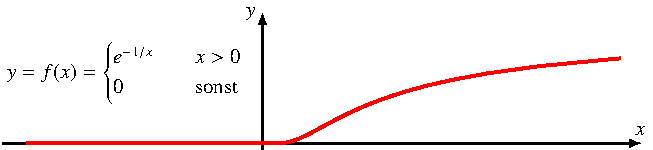
\includegraphics{chapters/020-variation/images/f.pdf}
\caption{Die beliebig oft stetig differenzierbare Funktion von
Satz~\ref{buch:variation:fundamentallemma:satz:glatt}
\label{buch:variation:fundamentallemma:fig:glatt}}
\end{figure}


\begin{satz}
\label{buch:variation:fundamentallemma:satz:glatt}
Die Funktion
\[
f(x)
=
\begin{cases}
e^{-1/x}&\qquad x>0\\
0&\qquad x\le 0
\end{cases}
\]
(siehe auch Abbildung~\ref{buch:variation:fundamentallemma:fig:glatt})
ist beliebig oft stetig differenzierbar.
\end{satz}

\begin{proof}
Es ist klar, dass die Funktion $f$ beliebig oft stetig differenzierbar
ist in jedem Punkt $x\ne 0$.
Es ist also nur nachzuweisen, dass $f(x)$ im Punkt $0$ beliebig
oft stetig differenzierbar ist.

Die ersten drei Ableitungen von $f(x)$ sind
\begin{align}
f'(x) &= \frac{1}{x^2} f(x)
\label{buch:variation:fundamentallemma:eqn:f1}
\\
f''(x) &= \frac{1-2x}{x^4}f(x)
\notag
\\
f'''(x) &= \frac{6x^2-6x+1}{x^6}f(x).
\notag
\end{align}
Daraus lässt sich die Vermutung ableiten, dass
\begin{equation}
f^{(n)}(x)
=
\frac{p_{n-1}(x)}{x^{2n}} f(x)
\label{buch:variation:fundamentallemma:eqn:fabl}
\end{equation}
ist, wobei $p_k(x)$ ein Polynom vom Grad $k$ ist.
Wir beweisen diese Vermutung mit Hilfe von vollständiger Induktion.
Die Induktionsverankerung für die $0$-te Ableitung ist trivial.

Wir nehmen jetzt im Sinne der Induktionsannahme an, dass die $n$-te
Ableitung die Form \eqref{buch:variation:fundamentallemma:eqn:fabl}
hat.
Wir müssen zeigen, dass dann auch $f^{(n+1)}(x)$ diese Form hat.
Dazu berechnen wir
\begin{align}
f^{(n+1)}(x)
&=
\frac{d}{dx}
\frac{p_n(x)}{x^{2n}} f(x)
\notag
\\
&=
\frac{p_n'(x)}{x^{2n}} f(x)
-2n
\frac{p_n(x)}{x^{2n+1}} f(x)
+
\frac{p_n(x)}{x^{2n}} f'(x).
\notag
\intertext{Mit der ersten Ableitung
\eqref{buch:variation:fundamentallemma:eqn:f1} wird dies zu}
&=
\frac{p_n'(x)}{x^{2n}} f(x)
-2n
\frac{p_n(x)}{x^{2n+1}} f(x)
+
\frac{p_n(x)}{x^{2n}} \frac{1}{x^2}f(x)
\notag
\\
&=
\frac{x^2p_n'(x) -2nxp_n(x)+p_n(x)}{x^{2n+2}} f(x).
\label{buch:variation:fundamentallemma:eqn:induktionsschritt}
\end{align}
Die Ableitung $p_n'(x)$ ist ein Polynom vom Grad $n-1$ und damit
ist $x^2p_n'(x)$ ein Polynom vom Grad $n+1$.
Ebenso ist $xp_n(x)$ ein Polynom vom Grad $n+1$ während
$p_n(x)$ ein Polynom vom Grad $n$ ist.
Der Zähler von
\eqref{buch:variation:fundamentallemma:eqn:induktionsschritt}
ist
\[
p_{n+1}(x)
=
x^2p_n'(x)+(1 -2nx)p_n(x),
\]
ein Polynom vom Grad $n+1$.
Damit ist der Induktionsschritt erfolgreich und die Behauptung betreffend
die Form von $f^{(n)}(x)$ ist bewiesen.

Es ist jetzt nur noch zu zeigen, dass der Grenzwert von $f^{(n)}(x)$
für $x\to 0+$ verschwindet.
Da das Polynom $p_n(x)$ stetig ist, folgt
\[
\lim_{x\to 0}
f^{(n)}(x)
=
\lim_{x\to 0}\frac{p_n(x)}{x^{2n}}f(x)
=
p_n(0) \lim_{t\to\infty} t^{2n} e^{-t}
=
0.
\]
Damit ist die beliebige stetige Differenzierbarkeit an der Stelle
$x=0$ gezeigt.
\end{proof}

Die Funktion $f(x)$ von 
Satz~\ref{buch:variation:fundamentallemma:satz:glatt} 
erfüllt noch nicht die Forderung, dass sie nur in einem vorgegebenen
Intervall von $0$ verschieden ist.

%
% g.tex -- template for standalon tikz images
%
% (c) 2021 Prof Dr Andreas Müller, OST Ostschweizer Fachhochschule
%
\documentclass[tikz]{standalone}
\usepackage{amsmath}
\usepackage{times}
\usepackage{txfonts}
\usepackage{pgfplots}
\usepackage{csvsimple}
\usetikzlibrary{arrows,intersections,math}
\begin{document}
\def\skala{3}
\def\a{-0.5}
\def\b{2.5}
\pgfmathparse{2/(\b-\a)}
\xdef\l{\pgfmathresult}
\begin{tikzpicture}[>=latex,thick,scale=\skala]

\draw[->] (-1,0) -- (3,0) coordinate[label={$x$}];
\draw[->] (0,-0.05) -- (0,1.1) coordinate[label={left:$y$}];

\begin{scope}
\clip (-1,-0.1) rectangle (2.9,1);
\draw[color=red,line width=1.2pt]
	plot[domain=0.25:10,samples=100] ({\a+1/\x},{exp(-\x)})
	-- (\a,0) -- (-1,0);
\draw[color=red,line width=1.2pt]
	plot[domain=0.25:10,samples=100] ({\b-1/\x},{exp(-\x)})
	-- (\b,0) -- (3,0);

\draw[color=blue,line width=1.2pt]
	plot[domain=\l:10,samples=100]
		({\a+1/\x},{exp(-\x)*exp(-1/(\b-\a-1/\x))}) -- (\a,0) -- (-1,0);
\draw[color=blue,line width=1.2pt]
	plot[domain=\l:10,samples=100]
		({\b-1/\x},{exp(-\x)*exp(-1/(-\a+\b-1/\x))}) -- (\b,0) -- (3,0);
\end{scope}

\draw (\a,-0.02) -- (\a,0.02);
\node at (\a,0) [below] {$a\mathstrut$};
\draw (\b,-0.02) -- (\b,0.02);
\node at (\b,0) [below] {$b\mathstrut$};
\node[color=blue] at ({0.5*(\a+\b)},0.12) {$g_{a,b}(x)$};
\node[color=red] at (\a,0.8) {$f(x-a)\mathstrut$};
\node[color=red] at (\b,0.8) {$f(b-x)\mathstrut$};

\end{tikzpicture}
\end{document}



\begin{satz}
\label{buch:variation:fundamentallemma:satz:gab}
Sei $f(x)$ die Funktion von
Satz~\ref{buch:variation:fundamentallemma:satz:glatt}.
Dann ist
\[
g_{a,b}(x)
=
f(x-a) f(b-x)
\]
eine unendlich oft stetig differenzierbare, nichtnegative Funktion mit Träger
$\supp g_{a,b}=(a,b)$.
\end{satz}

Die Funktionen $g_{a,b}(x)$ sind beliebig oft differenzierbar und nur im
Intervall $[a,b]$ von $0$ verschieden und sogar positiv.
Weil sie stetig sind, sind sie auch integrierbar, man kann also das
Integral über $\mathbb{R}$ berechnen und die Funktion damit normieren.
Die neue Funktion
\[
\frac{1}{N}
\tilde{g}_{a,b}(x)
\qquad\text{mit}\;
N
=
\int_{-\infty}^{\infty}g_{a,b}(x)\,dx
=
\int_a^b g_{a,b}(x)\,dx
\]
ist immer noch beliebig oft stetig differenzierbar und hat zusätzlich die
Eigenschaft
\[
\int_{-\infty}^{\infty}
\tilde{g}_{a,b}(x)\,dx
=
\int_a^b
\tilde{g}_{a,b}(x)\,dx
=
1.
\]
Wir formulieren dieses Resultat als Satz.

\begin{satz}
\label{buch:variation:satz:gabeins}
Zu jedem Intervall $[a,b]$ gibt es eine beliebig oft stetig
differenzierbare Funktion $g(x)$, genau das Intervall $[a,b]$
als Träger hat und deren Integral über $[a,b]$ den Wert $1$ hat.
\end{satz}

%
% Das Fundamentallemma
%
\subsection{Das Fundamentallemma}
Mit der Funktion $g_{a,b}(x)$ von
Satz~\ref{buch:variation:fundamentallemma:satz:gab}
lässt sich jetzt das Fundamentallemma in der folgenden Form
leicht beweisen.

\begin{satz}[Fundamentallemma]
\label{buch:variation:fundamentallemma:satz:fundamentallemma}
Wenn für die stetige Funktion $f\colon[a,b]\to\mathbb{R}$ 
\begin{equation}
\int_a^b f(x)\varphi(x)\,dx = 0
\label{buch:variation:fundamentallemma:eqn:fundamentalbed}
\end{equation}
gilt für jede beliebig oft stetig differenzierbare Funktion $\varphi(x)$ 
dann ist $f(x)=0$.
Das Resultat gilt selbst dann, wenn
\eqref{buch:variation:fundamentallemma:eqn:fundamentalbed}
nur für beliebig oft stetig differenzierbare Funktionen $\varphi(x)$ 
gilt, die ausserdem an den Intervallenden verschwinden:
$\varphi(a)=\varphi(b)=0$.
\end{satz}

\begin{proof}
Wir zeigen mit Hilfe eines Widerspruchs, dass es keinen Punkt $x_0\in[a,b]$
geben kann, für den $f(x_0)\ne 0$ ist.
Dazu nehmen wir also an, dass $f(x_0)\ne 0$ ist.
Falls $f(x_0)<0$ ist, ersetzen wir $f$ durch $-f$, 
die Bedingung
\eqref{buch:variation:fundamentallemma:eqn:fundamentalbed}
ändert sich dadurch nicht.
%
% fundamentallemma.tex -- Fundamentallemma
%
% (c) 2021 Prof Dr Andreas Müller, OST Ostschweizer Fachhochschule
%
\documentclass[tikz]{standalone}
\usepackage{amsmath}
\usepackage{times}
\usepackage{txfonts}
\usepackage{pgfplots}
\usepackage{csvsimple}
\usetikzlibrary{arrows,intersections,math}
\definecolor{darkgreen}{rgb}{0.0,0.6,0.0}
\definecolor{darkred}{rgb}{0.8,0.0,0.0}
\begin{document}
\def\skala{1}
\def\X{4.555}
\def\X{4.7}
\def\e{0.85}
\begin{tikzpicture}[>=latex,thick,scale=\skala,
declare function={
	f(\t) = (-0.4*\t)+4-1.5*sin(50*\t)-1.5*cos(120*\t);
}]

\fill[color=darkred!20]
	plot[domain=-180:180] ({\X+\e*\x/180},{cos(\x)+1})
	--
	cycle;

\draw[color=blue!20,line width=1.2pt]
	plot[domain=0.2:7.8,samples=100] ({\x},{f(\x)});
\begin{scope}
\clip ({\X-\e},0) rectangle ({\X+\e},5.4);
\draw[color=blue,line width=1.4pt]
	plot[domain={\X-2*\e}:{\X+2*\e},samples=100] ({\x},{f(\x)});
\end{scope}
\node[color=blue] at ({\X-0.8*\e},{f(\X-0.8*\e)}) [left] {$f(x)$};
%\node[color=blue] at ({\X},{f(\X)}) [above] {$f(x_0)$};
\draw[color=blue,line width=0.4pt] (0,{f(\X)}) -- ({\X},{f(\X)});
\draw[color=blue] (-0.05,{f(\X)}) -- (0.05,{f(\X)});
\node[color=blue] at (-0.05,{f(\X)}) [left] {$f(x_0)$};

\draw[color=blue,line width=0.4pt] ({\X},0) -- ({\X},{f(\X)});
\node at (\X,-0.05) [below] {$x_0\mathstrut$};

\draw[color=darkgreen,line width=0.4pt] ({\X-\e},0) -- ({\X-\e},5.2);
\draw[color=darkgreen,line width=0.4pt] ({\X+\e},0) -- ({\X+\e},5.2);
\draw[color=darkgreen,line width=0.4pt] (0,{0.5*f(\X)}) -- ({\X},{0.5*f(\X)});
\draw[color=darkgreen] (-0.05,{0.5*f(\X)}) -- (0.05,{0.5*f(\X)});
\node[color=darkgreen] at (-0.05,{0.5*f(\X)})
	[left] {$\frac12f(x_0)\mathstrut$};
\draw[color=darkgreen,line width=1.2pt]
	({\X+\e},{0.5*f(\X)}) 
	-- 
	({\X-\e},{0.5*f(\X)});
%\node[color=darkgreen] at ({\X},{0.5*f(\X)}) [above] {$\frac12f(x_0)$};
\draw[color=darkgreen] ({\X-\e},-0.05) -- ({\X-\e},0.05);
\node[color=darkgreen] at ({\X-\e},-0.05) [below left] {$x_0-\delta\mathstrut$};
\draw[color=darkgreen] ({\X+\e},-0.05) -- ({\X+\e},0.05);
\node[color=darkgreen] at ({\X+\e},-0.05) [below right] {$x_0+\delta\mathstrut$};

\fill[color=blue] ({\X},{f(\X)}) circle[radius=0.08];

\draw[->] (-0.1,0) -- (8.5,0) coordinate[label={$x$}];
\draw[->] (0,-0.1) -- (0,5.4) coordinate[label={left:$y$}];

\draw[color=darkred,line width=1.2pt]
	(0.5,0)
	--
	({\X-\e},0)
	--
	plot[domain=-180:180] ({\X+\e*\x/180},{cos(\x)+1})
	--
	({\X+\e},0)
	--
	(7.5,0);
\node[color=darkred] at ({\X+0.5*\e},1) [right] {$g(x)$};

\draw[line width=0.4pt] (0.5,0) -- (0.5,5.2);
\draw (0.5,-0.05) -- (0.5,0.05);
\node at (0.5,-0.05) [below] {$x_1\mathstrut$};

\draw[line width=0.4pt] (7.5,0) -- (7.5,5.2);
\draw (7.5,-0.05) -- (7.5,0.05);
\node at (7.5,-0.05) [below] {$x_2\mathstrut$};

\end{tikzpicture}
\end{document}


Wir dürfen daher annehmen, dass $f(x_0)>0$ ist
(Abbildung~\ref{buch:variation:fundamentallemma:fig:beweis}).
Da $f$ stetig ist, gibt es ein Intervall $[x_0-\varepsilon,x_0+\varepsilon]$
derart, dass $f(x)> \frac12 f(x_0)$ für
$x\in[x_0-\varepsilon,x_0+\varepsilon]$ gilt.
Dann gilt für das Integral
\[
\int_a^b
f(x)
g_{x_0-\varepsilon,x_0+\varepsilon} (x)
\,dx
>
\frac{f(x_0)}{2}
\int_a^b
g_{x_0-\varepsilon,x_0+\varepsilon} (x)
\,dx
>
0
\]
im Widerspruch zur Bedingung
\eqref{buch:variation:fundamentallemma:eqn:fundamentalbed}.
Der Widerspruch zeigt, dass $f(x)=0$ sein muss.
\end{proof}

%
% Skalarproduktformulierung des Fundamentallemmas
%
\subsection{Skalaproduktformulierung des Fundamentallemmas}
Die Richtungsableitung einer Funktion endlich vieler Variablen 
konnte als Skalarprodukt mit dem Gradienten geschrieben werden und
das Fundamentallemma hat besagt, dass der Gradient verschwindet,
wenn alle Richtungsableitungen verschwinden.
Diese Schlussweise ist auch für Funktionen möglich, wenn man Funktionen
ein Skalarprodukt definieren kann.

\begin{definition}[$L^2$-Skalarprodukt]
Das {\em Skalarprodukt} zweier quadratintegrierbarer Funktion $f$ und $g$
auf dem Intervall $[a,b]$ ist definiert durch
\[
\langle f,g\rangle
=
\int_a^b f(x)g(x)\,dx.
\]
\end{definition}

\begin{satz}[Fundamentallemma, Skalarproduktform]
Wenn für eine stetige Funktion $f\colon[a,b]\to\mathbb{R}$ das Skalarprodukt
\[
\langle f,\varphi\rangle = 0
\]
ist für jede unendlich oft differenzierbare Funktion $\varphi$ auf dem
Intervall $[a,b]$, dann ist $f=0$.
\end{satz}



%
% 3-eulerlagrange.tex
%
% (c) 2023 Prof Dr Andreas Müller
%
\section{Die Euler-Lagrange Differentialgleichung
\label{buch:variation:section:eulerlagrange}}
\kopfrechts{Die Euler-Lagrange Differentialgleichung}
Das Neuartige an der Aufgabenstellung des Brachistochronenproblems
war, dass eine Funktion gesucht war, so dass ein damit gebildetes
Integral eine Minimaleigenschaft erfüllt.
Für die damalige Mathematik war die Aufgabe, eine Funktion zu finden,
nicht neu.
Die Theorie der Differentialgleichungen war bereits entwickelt,
Newton hat die Infinitesimalrechnung ja erfunden, um damit die
Bewegungsgleichungen der Physik zu formulieren und zu lösen.
In einer Differentialgleichung werden Werte und Ableitungen einer
Funktion an einer einzigen Stelle miteinander verbunden.
Etwas salop formuliert sagt die Differentialgleichung in jedem
Punkt, in welche Richtung und mit welcher Krümmung die Funktionskurve
weiter zu zeichnen ist.

Im Brachistochronenproblem tragen aber alle Werte der gesuchten
Funktion zum Integral bei, es scheint daher auf den ersten Blick
nicht möglich, das Problem durch schrittweise Konstruktion
``von Punkt zu Punkt'' der Lösungskurve zu konstruieren.

Bernoullis Lösung des Brachistochrononproblems beruht auf der
Beobachtung, dass sich die Bedinung für die schnellste Bahn
durch eine Bedingung ersetzen lässt, die in jedem einzelnen
Punkt ausgewertet werden kann.
Das von ihm verwendete Fermat-Prinzip wurde ursprünglich ebenfalls
als eine globale Eigenschaft eines Lichtstrahls formuliert.
Aus dem Fermat-Prinzip folgt aber das Brechungsgesetz, welches
sagt, dass die Richtung eines Strahls in einem Punkt genau dann
ändert, wenn sich dort auch der Brechungsindex der beiden Medien
ändert.
Das Fermat-Prinzip ist also ein Beispiel dafür, wie eine globale
Bedingung erfüllt werden kann, indem einer lokalen Regel in jedem
Punkt gefolgt wird.

Es ist das Verdienst von Euler und Lagrange, zu erkennen, dass diese
Übersetzung eines globalen Variationsproblems in ein lokales 
Problem immer möglich ist.
Es entsteht dabei die Euler-Lagrange-Differentialgleichung, welche
die Problemstellung auf die Lösung einer Differentialgleichung
reduziert.
Damit ist ein allgemein anwendbares Lösungsverfahren gefunden.
Zu einem Variationsproblem lässt sich immer eine Differentialgleichung
finden, welche die gesuchte Funktion als Lösung hat.

In diesem Abschnitt soll dieser indirekte Weg der Lösung von
Variationsaufgaben dargestellt werden.
Wir werden später zeigen, dass diese Vorgehensweise nicht immer
erfolgreich sein kann.
Zum Beispiel werden wir in Kapitel~\ref{buch:chapter:nichtdiff}
Variationsprobleme kennenlernen, deren Lösungskurven nicht
differenzierbar sind und daher auch nicht von einer Differentialgleichung
gefunden werden können.
Im Kapitel~\ref{buch:chapter:direkt} werden daher die sogenannten
direkten Methodn vorgestellt, die den Umweg über eine
Differentialgleichung vermeiden.

%
% Die Lagrange-Funktion
%
\subsection{Die Lagrange-Funktion
\label{buch:variation:eulerlagrange:subsection:lagrange-funktion}}
Wir betrachten Variationsproblem der folgenden Art.
Gesucht ist eine auf dem Intervall $[x_0,x_1]$ definirte
Funktion $y(x)$, die das Integral
\begin{equation}
I(y)
=
\int_{x_0}^{x_1}
F(x, y(x), y'(x))
\,dx
\label{buch:variation:eulerlagrange:eqn:funktional}
\end{equation}
maximiert oder minimiert.
Der Ausdruck~\eqref{buch:variation:eulerlagrange:eqn:funktional}
wird ein Funktional genannt.
Die Funktion
\[
F
\colon
\mathbb{R}\times
\mathbb{R}\times
\mathbb{R}
\to
\mathbb{R}
\]
von drei Variablen heisst die {\em Lagrange-Funktion}
des Funktionals \eqref{buch:variation:eulerlagrange:eqn:funktional}.

\begin{beispiel}
Die Lagrange-Funktion des Brachistochronenproblems ist
\[
F(x,y,y')
=
\sqrt{ \frac{1+y^{\prime 2}}{y} }.
\]
Die Funktion hängt nicht von $x$ ab, was bedeutet, dass eine
Verschiebung in $x$-Richtung die Form der Lösungsfunktion des
Variationsproblems nicht ändert.
\end{beispiel}

\begin{beispiel}
\label{buch:variation:eulerlagrange:beispiel:gerade}
Wir formulieren die Aufgabe, die kürzeste Verbindung der Punkte
$(x_0,y_0)$ und $(x_1,y_1)$ in einer Ebene zu finden, als Variationsproblem.
Die Länge einer Kurve $y(x)$ ist das Integral
\[
l(y)
=
\int_{x_0}^{x_1}
\sqrt{1+y'(x)^2}\,dx.
\]
Daraus lesen wir ab, dass die Lagrange-Funktion dieses Variationsproblems
\begin{equation}
F(x,y,y') = \sqrt{1+y^{\prime 2}}
\label{buch:variation:eulerlagrange:eqn:geradeL}
\end{equation}
ist.
Die Funktion hängt weder von $x$ noch von $y$ ab.
Dies ist auch zu erwarten, denn die Länge einer Kurve hängt nicht davon
ob, wo in der Ebene sie platziert ist.
Eine Verschiebung in $x$-Richtung würde das $x$-Argument ändern,
eine Verschiebung in $y$-Richtung die $y$-Werte.
Wäre $F$ von $x$ oder $y$ abhängig, könnte auch die Länge der Kurve
davon abhängen.
\end{beispiel}

%
% Euler-Lagrange_Differentialgleichung
%
\subsection{Euler-Lagrange-Differentialgleichung
\label{buch:variation:eulerlagrange:subsection:dgl}}
%
% variation0.tex -- Variation mit festen Enden
%
% (c) 2021 Prof Dr Andreas Müller, OST Ostschweizer Fachhochschule
%
\documentclass[tikz]{standalone}
\usepackage{amsmath}
\usepackage{times}
\usepackage{txfonts}
\usepackage{pgfplots}
\usepackage{csvsimple}
\usetikzlibrary{arrows,intersections,math}
\definecolor{darkred}{rgb}{0.8,0,0}
\begin{document}
\def\skala{1}
\def\xzero{1}
\def\xone{10}
\def\yzero{1}
\def\yone{5}
\begin{tikzpicture}[>=latex,thick,scale=\skala,
declare function={
	x(\t)   = (1-\t)*\xzero+\t*\xone;
	t(\x)   = (\x-\xzero)/(\xone-\xzero);
	eta(\t) = \t*(1-\t)*(2*cos(180*\t)+4*\t*sin(720*\t)+6);
	y(\t)   = (1-\t)*\yzero+\t*\yone+4*\t*(1-\t);
}]

\draw (\xzero,-0.05) -- (\xzero,0.05);
\draw (-0.05,\yzero) -- (0.05,\yzero);
\draw[line width=0.2pt] (\xzero,0) -- (\xzero,\yzero);
\draw[line width=0.2pt] (0,\yzero) -- (\xzero,\yzero);
\node at (\xzero,-0.05) [below] {$x_1\mathstrut$};
\node at (-0.05,\yzero) [left] {$y_1\mathstrut$};

\draw (\xone,-0.05) -- (\xone,0.05);
\draw (-0.05,\yone) -- (0.05,\yone);
\draw[line width=0.2pt] (\xone,0) -- (\xone,\yone);
\draw[line width=0.2pt] (0,\yone) -- (\xone,\yone);
\node at (\xone,-0.05) [below] {$x_2\mathstrut$};
\node at (-0.05,\yone) [left] {$y_2\mathstrut$};

\fill[color=darkred] (\xzero,\yzero) circle[radius=0.08];
\fill[color=darkred] (\xone,\yone) circle[radius=0.08];
\node at (\xzero,\yzero) [above left] {$P_1$};
\node at (\xone,\yone) [right] {$P_2$};

\foreach \e in {-1.6,-1.2,...,1.7}{
	\draw[color=gray,smooth] plot[domain=0:1] ({x(\x)},{y(\x)+\e*eta(\x)});
}
\node[color=gray] at (3.6,5.65) {$y(x)+\varepsilon\eta(x)$};

\draw[color=darkred,smooth,line width=1.4pt] plot[domain=0:1] ({x(\x)},{y(\x)});
\node[color=darkred] at (6.8,4.8) {$y(x)$};

\draw[->] (-0.1,0) -- (11.6,0) coordinate[label={$x$}];
\draw[->] (0,-0.1) -- (0,8) coordinate[label={right:$y$}];

\end{tikzpicture}
\end{document}


Das Maximum oder Minimum einer Funktionen mehrere Variablen wurde
gefunden, indem die Richtungsableitung berechnet und $=0$ gesetzt
wurde.
Um die Funktion zu bestimmen, die ein Funktional $I(y)$ zu einem
Maximum oder Minimum macht, versuchen wir, die Idee der Richtungsableitung
für ein Funktional nachzuahmen.
Wir nehmen daher an, dass $y(x)$ eine Funktion ist, die das Funktional
$I(y)$ zu einem Minimum macht.
Für die Richtungsableitung addieren wir ein Vielfaches einer
Funktion $\eta(x)$, die Summe $y(x)+\varepsilon\eta(x)$ entspricht
dann einer Geraden mit Richtung $\eta(x)$ im Funktionenraum
(Abbildung~\ref{buch:variation:fig:variation0}).
Die Funktionen $y(x)+\varepsilon\eta(x)$ sind aber nur dann Kandidaten
für eine Lösung des Problems, wenn immer noch
\begin{align*}
y(x_0) + \varepsilon \eta(x_0) &= y_0
&&\text{und}&
y(x_1) + \varepsilon \eta(x_1) &= y_1
\end{align*}
gilt.
Dies ist nur möglich, wenn $\eta(x_0)=\eta(x_1)=0$ ist.

Wir berechnen jetzt die Ableitung der Funktion
$\varepsilon\mapsto I(y+\varepsilon\eta )$ an der Stelle $\varepsilon=0$.
Da die Intervallgrenzen nicht von $\varepsilon$ abhängen, können wir
die Ableitung unter das Integral nehmen:
\begin{align*}
\frac{d}{d\varepsilon}
I(y+\varepsilon\eta)
&=
\int_{x_0}^{x_1}
\frac{d}{d\varepsilon}
F(x,y(x)+\varepsilon\eta(x),y(x)+\varepsilon\eta'(x))
\,dx.
\intertext{Da $F$ differenzierbar ist, kann die Ableitung mit der
Kettenregel berechnet werden, sie ist}
&=
\int_{x_0}^{x_1}
\frac{\partial F}{\partial y}
(x,y(x)+\varepsilon\eta(x),y(x)+\varepsilon\eta'(x))
\eta(x)
\\
&\qquad
+
\frac{\partial F}{\partial y'}
(x,y(x)+\varepsilon\eta(x),y(x)+\varepsilon\eta'(x))
\eta'(x)
\,dx.
\intertext{Uns interessiert aber nur der Wert an der Stelle $\varepsilon=0$,
er ist}
\frac{d}{d\varepsilon}
I(y+\varepsilon\eta)
\bigg|_{\varepsilon=0}
&=
\int_{x_0}^{x_1}
\frac{\partial F}{\partial y}
(x,y(x),y'(x))
\,
\eta(x)
+
\frac{\partial F}{\partial y'}
(x,y(x),y'(x))
\,
\eta'(x)
\,dx
=0.
\end{align*}
Das Integral hängt von den verschiedenen Faktoren $\eta(x)$ und
von $\eta'(x)$ in den beiden Termen unter dem Integral ab.
Wir integrieren den zweiten Term partiell 
\begin{align*}
\int_{x_0}^{x_1}
\frac{\partial F}{\partial y'}(x,y(x),y'(x))\,\eta'(x)\,dx
&=
\biggl[
\frac{\partial F}{\partial y'}(x,y(x),y'(x))\,\eta(x)
\biggr]_{x_0}^{x_1}
\\
&\qquad
-
\int_{x_0}^{x_1}
\frac{d}{dx}
\frac{\partial F}{\partial y'}(x,y(x),y'(x))\,\eta(x)\,dx.
\end{align*}
Da $\eta(x_0)=\eta(x_1)=0$ verschwindet der erste Term
auf der rechten Seite, es bleibt
\[
\frac{d}{d\varepsilon}
I(y+\varepsilon\eta)
\bigg|_{\varepsilon=0}
=
\int_{x_0}^{x_1}
\biggl(
\frac{\partial F}{\partial y}
(x,y(x),y'(x))
-
\frac{d}{dx}
\frac{\partial F}{\partial y'}
(x,y(x),y'(x))
\biggr)
\eta(x)
\,dx.
\]
Dies kann auch als Skalarprodukt
\[
\biggl\langle 
\frac{\partial F}{\partial y}
(x,y(x),y'(x))
-
\frac{d}{dx}
\frac{\partial F}{\partial y'}
(x,y(x),y'(x))
,
\eta(x)
\biggr\rangle
=
0
\]
geschrieben werden.
Da dies für jede differenzierbare Funktion $\eta$ mit Randwerten
$\eta(x_0)=\eta(x_1)$ gelten muss, folgt nach dem
Fundamentallemma~\ref{buch:variation:fundamentallemma:satz:fundamentallemma},
der folgende Satz. 

\begin{satz}[Euler-Lagrange]
\label{buch:variation:eulerlagrange:satz:eulerlagrange}
Wenn die mindestens zweimal stetig differenzierbare Funktion $y(x)$
unter allen solchen Funktionen mit $y(x_0)=y_0$ und $y(x_1)=y_1$
das Funktional
\[
I(y)
=
\int_{x_0}^{x_1}
F(x,y(x),y'(x))\,dx
\]
zu einem Maximum oder Minimum macht, dann ist $y(x)$ eine Lösung der
gewöhnlichen Differentialgleichung
\begin{equation}
\frac{d}{dx}
\frac{\partial F}{\partial y'}(x,y(x),y'(x))
-
\frac{\partial F}{\partial y}(x,y(x),y'(x))
=
0.
\label{buch:variation:eulerlagrange:eqn:eulerlagrange}
\end{equation}
Sie heisst die {\em Euler-Lagrange-Differentialgleichung}.
\end{satz}

Eine Lösung des Variationsproblems kann also als Lösung der
Euler-Lagrange-Dif\-fe\-ren\-tial\-glei\-chung mit den Randwerten
$y(x_0)=x_0$ und $y(x_1)=y_1$ gefunden werden.
Die Bedingung ist notwendig, aber nicht hinreichend.
Wie bei der Bestimmung eines Extremums bei Funktionen endlich
vieler Variablen garantiert das Verschwinden der Richtungsableitung
nicht, dass auch tatsächlich ein Extremum vorliegt.
Man sagt daher auch, dass eine Lösung $y(x)$ der
Euler-Lagrange-Differentialgleichung das Funktional $I(y)$
stationär macht.

Eine weitere Einschränkung ist, dass die Herleitung der
Euler-Lagrange-Differential\-gleichung vorausgesetzt hat,
dass die Lösungsfunktion $y(x)$ mindestens zweimal 
stetig differenzierbar ist.
Es gibt aber durchaus Variationsprobleme, deren Lösungen
nicht differenzierbar sind, dazu mehr im Kapitel~\ref{buch:chapter:nichtdiff}.

\begin{beispiel}
\label{buch:variation:eulerlagrange:beispiel:gerade}
Wir lösen das Variationsproblem von Beispiel
\ref{buch:variation:eulerlagrange:beispiel:gerade}
mit der Lagrange-Funk\-tion
\eqref{buch:variation:eulerlagrange:eqn:geradeL}.
Da die Lagrange-Funktion nicht von $y$ abhängt, bleibt von der 
Euler-Lagrange-Gleichung nur
\[
\frac{d}{dx}
\frac{\partial L}{\partial y'}(x,y(x),y'(x))
=
0
\]
übrig.
Berechnung der Ableitung liefert
\begin{equation}
\frac{\partial}{\partial y'}
\sqrt{1+y^{\prime 2}}
=
\frac{y'}{\sqrt{1+y^{\prime 2}}}.
\label{buch:variation:eulerlagrange:eqn:ableitungFyp}
\end{equation}
Die Ableitung nach $x$ ergibt
\begin{align*}
\frac{d}{dx}
\frac{\partial}{\partial y'}
\sqrt{1+y^{\prime 2}}
&=
\frac{d}{dx}
\frac{y'}{\sqrt{1+y^{\prime 2}}}
\\
&=
\frac{
y''\sqrt{1+y^{\prime 2}}-y'\cdot \frac{y'y''}{\sqrt{1+y^{\prime 2}}}
}{
1+y^{\prime 2}
}
\\
&=
y''
\frac{
1+y^{\prime 2}-y^{\prime 2}
}{
(1+y^{\prime 2})^{\frac32}
}.
\intertext{Die Euler-Lagrange-Differentialgleichung ist daher}
0
&=
\frac{y''}{(1+y^{\prime 2})^{\frac32}} .
\end{align*}
Der Nenner auf der rechten Seite ist immer $\ge 1$, die Gleichung kann
also nur erfüllt sein, wenn $y''=0$ ist.
Die Funktion $y(x)$ muss also eine lineare Funktion $y=ax+b$ sein.
Die Randbedingung wird erfüllt für die Geradengleichung
\[
y(x)
=
\frac{y_1-y_0}{x_1-x_0}(x-x_0) + y_0.
\]
Kürzeste Verbindungen in der Ebene sind daher Geraden.
\end{beispiel}

%
% Freie Randbedingungen
%
\subsection{Freie Randbedingungen
\label{buch:variation:eulerlagrange:subsection:freierb}}
In der Herleitung der Euler-Lagrange-Differentialgleichung wurde angenommen,
dass die Endpunkte der Lösungsfunktion durch $y(x_0)=y_0$ und $y(x_1)=y_1$
fest vorgegeben sind.
Diese Voraussetzung soll in diesem Abschnitt abgeschwächt werden.
Die Funktionswerte in den Endpunkten sollen also nicht mehr fest
vorgegeben sein.

\begin{beispiel}
\label{buch:variation:eulerlagrange:beispiel:freiegerade}
Im Beispiel~\ref{buch:variation:eulerlagrange:beispiel:gerade}
wurde die kürzeste Kurve zwischen zwei Punkten in der Ebene
gesucht und wie erwartet eine Gerade als Lösung gefunden.
Wenn die Werte $y_0$ und $y_1$ jetzt nicht mehr vorgegeben sind,
wird die kürzeste Verbindung zwischen den beiden Geraden
$x=x_0$ und $x=x_1$ gesucht.
Die Lösung dieses Problems ist nicht eindeutig, jede horizontale
Strecke mit $y_0=y_1$ ist eine Lösung.
\end{beispiel}

Das Beispiel zeigt, dass es im Allgemeinen immer noch die Vorgabe
eines der beiden Randwerte braucht, um die Lösung eindeutig zu
bestimmen.
Wir lösen daher die folgende Aufgabe.

\begin{aufgabe}
Gesucht ist eine zweimal stetig differnzierbare Funktion $y(x)$ auf
dem Intervall $[x_0,x_1]$ mit $y(x_0)=y_0$, die das Integral
\[
I(y)
=
\int_{x_0}^{x_1} F(x,y(x),y'(x))\,dx
\]
zu einem Extremum macht.
Am rechten Ende des Intervalls ist der Funktion $y(x)$ keine
Randbedingung auferlegt.
\end{aufgabe}

\begin{proof}[Lösung]
%
% variation1.tex -- Variation mit freiem rechtem Ende
%
% (c) 2021 Prof Dr Andreas Müller, OST Ostschweizer Fachhochschule
%
\documentclass[tikz]{standalone}
\usepackage{amsmath}
\usepackage{times}
\usepackage{txfonts}
\usepackage{pgfplots}
\usepackage{csvsimple}
\usetikzlibrary{arrows,intersections,math}
\definecolor{darkred}{rgb}{0.8,0,0}
\begin{document}
\def\skala{1}
\def\xzero{1}
\def\xone{10}
\def\yzero{1}
\def\yone{4}
\begin{tikzpicture}[>=latex,thick,scale=\skala,
declare function={
	x(\t)   = (1-\t)*\xzero+\t*\xone;
	t(\x)   = (\x-\xzero)/(\xone-\xzero);
	eta(\t) = \t*(1-\t)*2*cos(180*\t)+0.5*sin(810*\t)+1.8*\t;
	y(\t)   = (1-\t)*\yzero+\t*\yone+4*\t*(1-\t);
}]

\draw (\xzero,-0.05) -- (\xzero,0.05);
\draw (-0.05,\yzero) -- (0.05,\yzero);
\draw[line width=0.2pt] (\xzero,0) -- (\xzero,\yzero);
\draw[line width=0.2pt] (0,\yzero) -- (\xzero,\yzero);
\node at (\xzero,-0.05) [below] {$x_0\mathstrut$};
\node at (-0.05,\yzero) [left] {$y_0\mathstrut$};

\draw (\xone,-0.05) -- (\xone,0.05);
\draw[line width=0.2pt] (\xone,0) -- (\xone,{y(1)+1.6*eta(1)});
\node at (\xone,-0.05) [below] {$x_1\mathstrut$};

\fill[color=darkred] (\xzero,\yzero) circle[radius=0.08];
\fill[color=darkred] (\xone,\yone) circle[radius=0.08];
\node at (\xzero,\yzero) [above left] {$P_0$};
\node at (\xone,\yone) [right] {$P_1$};

\foreach \e in {-1.6,-1.2,...,1.7}{
	\draw[color=gray,smooth] plot[domain=0:1] ({x(\x)},{y(\x)+\e*eta(\x)});
}
\node[color=gray] at (3.2,3.75) {$y(x)+\varepsilon\eta(x)$};

\draw[color=darkred,smooth,line width=1.4pt] plot[domain=0:1] ({x(\x)},{y(\x)});
\node[color=darkred] at (6.2,3.98) {$y(x)$};

\draw[->] (-0.1,0) -- (11.6,0) coordinate[label={$x$}];
\draw[->] (0,-0.1) -- (0,8) coordinate[label={right:$y$}];

\end{tikzpicture}
\end{document}


Sei $y(x)$ eine Lösung der Aufgabe und sei $y_1:=y(x_1)$ der Wert
der Lösung am rechten Rand des Intervalls.
Wir berechnen wieder die Variation von $I(y)$ mit Hilfe von
stetig differenzierbaren Funktionen $\eta(x)$, die jetzt aber 
nur noch die Bedingungn $\eta(x_0)=0$ erfüllen müssen
(Abbildung~\ref{buch:variation:fig:variation1}).
Die Richtungsableitung ist wie früher
\begin{align*}
\frac{d}{d\varepsilon}
I(y+\varepsilon\eta)
\bigg|_{\varepsilon=0}
&=
\frac{d}{d\varepsilon}
\int_{x_0}^{x_1}
F(x,y(x)+\varepsilon\eta(x),y'(x)+\varepsilon\eta'(x))\,dx
\\
&=
\int_{x_0}^{x_1}
\frac{\partial F}{\partial y}(x,y(x),y'(x)) 
\eta(x)
+
\frac{\partial F}{\partial y'}
(x,y(x),y'(x))
\eta'(x)
\,dx
\intertext{und mit partieller Integration}
&=
\biggl[
\frac{\partial F}{\partial y'}(x,y(x),y'(x)) \eta(x)
\biggr]_{x_0}^{x_1}
\\
&\qquad
+
\int_{x_0}^{x_1}
\biggl(
\frac{\partial F}{\partial y}(x,y(x),y'(x))
-
\frac{d}{dx}
\frac{\partial F}{\partial y'}(x,y(x),y'(x))
\biggr)
\,
\eta(x)
\,dx.
\end{align*}
Im Gegensatz zu früher können wir jetzt aber nicht mehr
schliessen, dass der erste Term verschwindet, da $y(x_1)$ nicht
mehr als $=0$ verausgesetzt wird.
Vielmehr erhalten wir für die erste Variation
\begin{equation*}
\delta I(y)
=
\frac{\partial F}{\partial y'} (x_1,y(x_1),y'(x_1)) \eta(x_1)+
\int_{x_0}^{x_1}
\biggl(
\frac{\partial F}{\partial y}(x,y(x),y'(x))
-
\frac{d}{dx}
\frac{\partial F}{\partial y'}(x,y(x),y'(x))
\biggr)
\,
\eta(x)
\,dx.
\end{equation*}
Die Klammer im Integral ist von der Euler-Lagrange-Differentialgleichung
her bekannt, aber es ist ein weiterer hinzugekommen, der genau dann
verschwindet wenn auch $\eta(x_1)=0$ ist.

Dann ist $y(x)$ natürlich erst recht eine Lösung des Problems, das
Funktional $I(y)$ mit den {\em zwei} Randbedingungen
$y(x_0)=y_0$ und $y(x_1)=y_1$ zu einem Extremum zu machen, also
muss die Funktion $y(x)$ sicher die Euler-Lagrange-Differentialgleichung
erfüllen.
Die Klammer im Integral wird daher verschwinden, die Variation
reduziert sich auf den ersten Term
\[
\delta I(y)
=
\frac{\partial F}{\partial y'} (x_1,y(x_1),y'(x_1)) \eta(x_1)
=
0.
\]
Sie verschwindet nur dann für alle zulässigen Funktionen $\eta(x)$, wenn
\begin{equation*}
\frac{\partial F}{\partial y'}(x_1,y(x_1),y'(x_1))=0
\end{equation*}
gilt.
Dies ist eine zusätzliche Randbedingung für die Funktion $y(x)$, geschrieben
in einer impliziten Form.
\end{proof}

Wir halten das Resultat der Aufgabenlösung als Satz fest:

\begin{satz}
\label{buch:variation:eulerlagrange:satz:zusaetzlicherb}
Wenn die zweimal stetig differenzierbare Funktion $y(x)$ mit dem
Randwert $y(x_0)=y_0$ das Integral
\[
I(y)
=
\int_{x_0}^{x_1} F(x,y(x),y'(x))\,dx
\]
zu einem Extremum macht, dann erfüllt sie am rechten Intervallende
die Randbedingung
\begin{equation}
\frac{\partial F}{\partial y'}(x_1,y(x_1),y'(x_1))=0.
\label{buch:variation:eulerlagrange:eqn:zusaetzlicherb}
\end{equation}
zusätzlich zur Euler-Lagrange-Gleichung für die Lagrange-Funktion $F$.
\end{satz}

\begin{beispiel}
\label{buch:variation:eulerlagrange:beispiel:einseitigegerade}
Wir betrachten wieder das Funktional
\[
I(y)
=
\int_{x_0}^{x_1}
\sqrt{1+y^{\prime 2}(x)}
\,dx
\]
mit der einzigen Randbedingung $y(x_0)=y_0$, der Funktionswert auf 
der rechten Seite ist nicht vorgebeben.
Der Satz~\eqref{buch:variation:eulerlagrange:satz:zusaetzlicherb}
besagt zunächst, dass die Lösungsfunktion wieder eine Gerade sein
muss, da die Euler-Lagrange-Gleichung erfüllt sein muss.
Zusätzlich muss aber auch die Randbedingung
\eqref{buch:variation:eulerlagrange:eqn:zusaetzlicherb}
am rechten Ende des Intervalls erfüllt sein.
Die Ableitung der Lagrange-Funktion ist in diesem Fall durch
\eqref{buch:variation:eulerlagrange:eqn:ableitungFyp}
gegeben, es muss also
\[
\frac{y'(x_1)}{\sqrt{1+y'(x_1)^2}}
=
0
\qquad\Rightarrow\qquad y'(x_1)=0
\]
gelten.
Die Lösung ist daher wie erwartet eine horizontale Strecke.
\end{beispiel}



%
% 4-splines.tex
%
% (c) 2023 Prof Dr Andreas Müller
%
\section{Spline-Interpolation
\label{buch:variation:section:splines}}
\kopfrechts{Spline-Interpolation}
In diesem Abschnitt soll eine Anwendung diskutiert werden, die grossen
Nutzen in der numerischen Mathematik bringt.
Es unterscheidet sich von früheren Beispielen dadurch, dass die
gesuchte Funktion nicht nur an den Intervallenden festgehalten wird,
sondern auch die Werte in Zwischenpunkten vorgeschrieben sind.

%
% Problemstellung
%
\subsection{Problemstellung}
Von einer Funktion sind die Werte 
$f_i=f(x_i)$ in den Stellen $x_0=a<x_1<\dots<x_n=b$ bekannt.
Man finde eine Interpolationsfunktion $g(x)$ derart, dass
\[
f(x_i) = g(x_i)
\quad
\forall i=0,\dots,n.
\]
Ausserdem soll der Funktionsgraph von $g(x)$ möglichst wenig Krümmung haben.
Da die Krümmung eines Graphen ist im Wesentlichen abhängig von der zweiten
Ableitung, wir verlangen daher, dass das Integral
\begin{equation}
I(g)
=
\int_a^b g''(x)^2\,dx
\label{buch:variation:spline:eqn:funktional}
\end{equation}
möglichst klein wird.
Eine solche Funktion heisst {\em Spline-Interpolationsfunktion}.

%
% Euler-Lagrange-Differentialgleichung
%
\subsection{Euler-Lagrange-Differentialgleichung}
Die Lagrange-Funktion des
Funktionals~\eqref{buch:variation:spline:eqn:funktional} ist
\[
L(x,y,y',y'') = y^{\prime\prime 2}.
\]
Für die Herleitung der Euler-Lagrange-Differentialgleichungen
dürfen jetzt aber nur Funktionen $\eta$ verwendet werden, die
in den Stellen $x_i$ verschwinden.
Die Variation ergibt
\begin{align*}
\delta I
&=
\frac{d}{dt}
\int_a^b (y''(x)+t\eta''(x))^2\,dx
\bigg|_{t=0}
\\
&=
\int_a^b 2y''(x)\eta''(x) \,dx.
\end{align*}
Da wir nur wissen, dass $y''(x)$ in den Teilintervallen $[x_i,x_{i+1}]$
differenzierbar ist, muss die partielle Integration auf diese
Teilintervalle beschränkt werden:
\begin{align*}
\delta I
&=
2
\sum_{i=0}^{n-1}
\int_{x_i}^{x_{i+1}} y''(x) \eta'(x)\,dx
=
2\sum_{i=0}^{n-1}\biggl[y''(x)\eta(x)\biggr]_{x_i}^{x_{i+1}}
-
2\sum_{i=0}^{n-1}\int_{x_i}^{x_{i+1}} y'''(x)\eta'(x)\,dx
\\
&=
-2y''(a)\eta'(a)
+\sum_{i=0}^{n-1}\bigl(y''(x_i-) -y''(x_i+)\bigr)\eta'(x_i)
+
2y''(b)\eta'(b)
-
2
\sum_{i=0}^{n-1}
\biggl[
y'''(x_i)\eta(x_i)
\biggr]_{x_i}^{x_{i+1}}
\\
&\qquad
+2
\sum_{i=0}^{n-1}
\int_{x_i}^{x_{i+1}} y''''(x)\eta(x)\,dx.
\end{align*}
Da $\eta$ in den Stützstellen verschwindet, ist diezweite Summe auf der
rechten Seite $=0$.
Die Variation kann nur für alle $\eta$ verschwinden, wenn die
Koeffizienten in der ersten Summe verschwinden, es folgt daher, dass
\[
y''(x_i-) = y''(x_i+) \quad\text{für alle $i$},
\]
die Funktion $y(x)$ ist also zweimal stetig differenzierbar auf dem
ganzen Intervall.
Aus dem Fundamentallemma angewandt auf die letzte Summe folgt, dass
$y''''(x)=0$ ist in jedem Teilintervall $[x_i,x_{i+1}]$.
Die Funktion $y(x)$ ist daher auf jedem solchen Teilintervall ein
kubisches Polynom.

\begin{verbatim}
- Problemstellung
- Euler-Lagrange-Differentialgleichung
- Lösung der Differntialgleichung
- Fehlerformel
\end{verbatim}

%
% 5-hoehereableitungen.tex
%
% (c) 2023 Prof Dr Andreas Müller
%
\section{Höhere Ableitungen
\label{buch:variation:section:hoehereableitungen}}
\kopfrechts{Höhere Ableitungen}
Das Beispiel der Spline-Interpolation hat gezeigt, dass es manchmal
nötig ist, höhere Ableitungen als die erste in einem Funktional
zu berücksichtigen.
In diesem Abschnitt werden weitere Beispiele dazu vorgestellt.

%
% Lagrange-Funktion mit höheren Ableitungen
%
\subsection{Lagrange-Funktion mit höheren Ableitungen}
Die Euler-Lagrange-Differentialgleichung wurde bisher für Funktionale
hergeletet, deren Lagrange-Funktion von $x$, der Funktion $y(x)$ und
der ersten Ableitung $y'(x)$ abhängen.

\begin{definition}
Eine Funktion $L(x,y,y',\dots,y^{(n)})$ heisst eine Lagrange-Funktion
der Ordnung $n$.
\index{Lagrange-Funktion $n$-ter Ordnung}%
\end{definition}

\begin{beispiel}
Das Variationsproblem für die Spline-Integration hat die Lagrange-Funktion
zweiter Ordnung
\[
L(x,y,y',y'') = y^{\prime\prime 2}
\]
verwendet.
\end{beispiel}

Ein elastischer Stab speichert bei Verbiegung Energie, deren Dichte
entlang des Stabes proportional zur Krümmung ist.
Ist $s\mapsto \gamma(s)\in\mathbb{R}^2$ eine differenzierbare
Parametrisierung einer ebenen Kurve, die die Form eines dünnen elastischen
Stabes beschreibt, dann ist die Gesamtenergie des Stabes gegeben durch
das Integral
\[
E
=
\int_a^b \kappa(s)^2 \,ds.
\]
Ist $s$ ein Bogenlängenparameter, also $|\dot{\gamma}(s)|=1$, dann ist
die Krümmung die zweite Ableitung, also
\[
I = \int_a^b \ddot{\gamma}(s)^2\,ds.
\]
Diese Parameterdarstellung ist aber nicht die Form, in der wir bis jetzt
Kurven in der Ebene beschreiben konnten.

Sei $y(x)$ eine Funktion, deren Graph einen elastisch verbogenen Stab
in der Ebene beschreibt.
Die Krümmung des Graphen kann nach
\[
\kappa(x)
=
\frac{y''(x)}{(1+y'(x)^2)^{\frac32}}
\]
berechnet werden.
Die Energie des Stabes wird dann
\[
E
=
\int_a^b \frac{y''(x)^2}{(1+y'(x)^2)^3}\,dx.
\]
Die Lagrange-Funktion des Problems der Biegung eines Stabes ist daher
\[
L(x,y,y',y'')
=
\frac{y^{\prime\prime 2}}{(1+y^{\prime 2})^3}.
\]

%
% Die verallgemeinerte Euler-Lagrange-Differentialgleichung
%
\subsection{Die verallgemeinerte Euler-Lagrange-Differentialgleichung}
Auch für ein Variationsproblem mit einer Lagrange-Funktion, die höhere
Ableitungen enthält, lässt sich mit der mehr oder weniger gleichen
Vorgehensweise eine Differentialgleichung für die gesuchte Funktion
$y(x)$ herleiten.
Wie schon im Beispiel zur Spline-Interpolation angedeutet, wird es
notwendig sein, mehrmals partiell zu integrieren.

Sei also $L(x,y,y',\dots,y^{(n)})$ eine Lagrange-Funktion $n$-ter Ordnung
und sei eine Funktion $y(x)$ gesucht, die ein kritischer Punkt des Integrals
\[
I
=
\int_a^b L(x,y(x),y'(x),\dots,y^{(n)}(x))\,dx
\]
ist.
Wir berechnen wieder die erste Variation mit Hilfe einer beliebig
oft differenzierbaren Funktion $\eta(x)$, welche in den Endpunkten
des Intervalls zusammen mit allen Ableitungen verschwindet.
Die Variation ist definiert als die Richtungsableitung in Richtung
von $\eta(x)$ als
\begin{align*}
\delta I
&=
\frac{d}{dt}
\int_a^b
L(x,y(x)+t\eta(x),y'(x)+t\eta'(x),\dots,y^{(n)}(x)+t\eta^{(n)}(x))
\,dx\biggl|_{t=0}.
\intertext{Durch Ableitung nach $t$ finden wir}
&=
\int_a^b
\frac{\partial L}{\partial y}(x,y(x),y'(x),\dots,y^{(n)}(x))
\eta(x)
+
\frac{\partial L}{\partial y'}(x,y(x),y'(x),\dots,y^{(n)}(x))
\eta'(x)
\\
&\qquad
+
\dots
+
\frac{\partial L}{\partial y^{(n)}}(x,y(x),y'(x),\dots,y^{(n)}(x))
\eta^{(n)}(x)
\,dx.
\end{align*}
Die Terme mit Ableitungen von $\eta(x)$ können durch partielle
Integration in Terme umgewandelt werden, die nur die Funktion 
$\eta(x)$ enthalten:
\begin{align*}
\delta I
&=
\int_a^b
\frac{\partial L}{\partial y^{(k)}}
(x,y(x),y'(x),\dots,y^{(n)}(x))
\eta^{(k)}(x)
\,dx
\\
&=
\biggl[
\frac{\partial L}{\partial y^{(k)}}
(x,y(x),y'(x),\dots,y^{(n)}(x))
\eta^{(k-1)}(x)
\biggr]_a^b
\\
&\qquad
-
\int_a^b
\frac{d}{dx}
\frac{\partial L}{\partial y^{(k)}}
(x,y(x),y'(x),\dots,y^{(n)}(x))
\eta^{(k-1)}(x)
\,dx.
\intertext{Da die Ableitungen von $\eta(x)$ in den Intevallenden
verschwinden, ist dies gleichbedeutend mit}
&=
-\int_a^b \frac{d}{dx} \frac{\partial L}{\partial y^{(k)}}
(x,y(x),y'(x),\dots,y^{(n)}(x))
\eta^{(k-1)}(x)
\,dx.
\intertext{Durch Iterieren dieser Rechnung erhalten wir}
&=
(-1)^{k}
\int_a^b
\frac{d^k}{dx^k}
\frac{\partial L}{\partial y^{(k)}}
(x,y(x),y'(x),\dots,y^{(n)}(x))
\eta(x)
\,dx.
\end{align*}
Die Variation kann jetzt als
\begin{align*}
\delta I
&=
\int_a^b
\biggl(
\frac{\partial L}{\partial y}
-
\frac{d}{dx}
\frac{\partial L}{\partial y'}
+
\frac{d^2}{dx^2}
\frac{\partial L}{\partial y''}
-
\dots
+
(-1)^n
\frac{d^n}{dx^n}
\frac{\partial L}{\partial y^{(n)}}
\biggr)
\eta(x)\,dx
\end{align*}
geschrieben werden.
Die Variation $\delta I$ muss für jede Wahl von $\eta(x)$ verschwinden,
daher folgt aus dem Fundamentallemma, dass $y(x)$ die Differentialgleichung
\begin{equation}
\frac{\partial L}{\partial y}
-
\frac{d}{dx}
\frac{\partial L}{\partial y'}
+
\frac{d^2}{dx^2}
\frac{\partial L}{\partial y''}
-
\dots
+
(-1)^n
\frac{d^n}{dx^n}
\frac{\partial L}{\partial y^{(n)}}
=
0
\label{buch:variation:hohere:eqn:eulerlagrange}
\end{equation}
erfüllen muss.
Man beachte, dass wir in dieser Rechnung stillschweigend annehmen,
dass die Funktion $y(x)$ genügend oft stetig differenzierbar ist,
so dass die einzelnen Terme der Differentialgleichung
\eqref{buch:variation:hohere:eqn:eulerlagrange} wohldefiniert sind.

\begin{satz}[Euler-Lagrange-Differentialgleichung]
Eine genügend oft differenzierbare Funktion $y(x)$ ist ein stationärer
Punkt des Integrals
\[
I
=
\int_a^b
L(x,y(x),y'(x),\dots,y^{(n)}(x))
\,dx
\]
mit der Lagrange-Funktion $n$-ter Ordnung $L(x,y,y',\dots,y^{(n)})$,
wenn sie die die Euler-Lagrange-Differentialgleichung
\eqref{buch:variation:hohere:eqn:eulerlagrange} erfüllt.
\end{satz}



%
% 6-mehrerefunktionen.tex
%
% (c) 2023 Prof Dr Andreas Müller
%
\section{Varationsproblem für mehrere Funktionen
\label{buch:variation:section:mehrerefunktionen}}
\kopfrechts{Mehrere Funktionen}

%
% Lagrange-Funktion für mehrere Funktionen
%
\subsection{Lagrange-Funktion für mehrere Funktionen}

%
% Die Euler-Lagrange-Differentialgleichung
%
\subsection{Die Euler-Lagrange-Differentialgleichung}
Für eine Lagrange-Funktion für $r$ Funktionen $y_1(x),\dots,y_r(x)$
lässt sich die Variation des Integrals
\[
I
=
\int_a^b L(x,y_1(x),y_1'(x),\dots,y_r(x),y_r'(x))\,dx
\]
ganz analog zur einer Lagrange-Funktion
mit nur einer Funktion berechnen.
Dazu verwenden wir Funktionen $\eta_1(x),\dots,\eta_r(x)$, die
in den Endpunkten verschwinden und berechnen die Variation
\begin{align}
\delta I
&=
\frac{d}{dt}
\int_a^b
L(x,y_1(x)+t\eta_1(x),y_1'(x)+t\eta_1'(x),\dots,
y_r(x)+t\eta_r(x),y_r'(x)+t\eta_r'(x))
\,dx
\bigg|_{t=0}
\notag
\\
&=
\int_a^b
\frac{\partial L}{\partial y_1}\eta_1(x)
+
\frac{\partial L}{\partial y'_1}\eta'_1(x)
+
\dots
\frac{\partial L}{\partial y_r}\eta_r(x)
+
\frac{\partial L}{\partial y'_r}\eta'_r(x)
\,dx
\notag
\intertext{Die Terme mit Ableitungen von $\eta'_i(x)$ können durch partielle
Integration umgeformt werden:}
&=
\int_a^b
\frac{\partial L}{\partial y_1}\eta_1(x)
+\dots+
\frac{\partial L}{\partial y_r}\eta_r(x)
\,dx
+
\biggl[
\frac{\partial L}{\partial y'_1}\eta_1(x)
+
\frac{\partial L}{\partial y'_r}\eta_r(x)
\biggr]_a^b
\\
&\qquad
-
\int_a^b
\frac{d}{dx}
\frac{\partial L}{\partial y'_1}
\eta_1(x)
+
\dots
+
\frac{d}{dx}
\frac{\partial L}{\partial y'_r}
\eta_r(x).
\notag
\intertext{Der mittlere Term verschwindet, weil die Funktionen
$\eta_i(x)$ an den Intervallenden verschwinden.
Die Variation ist daher}
\delta I
&=
\int_a^b
\biggl(
\frac{\partial L}{\partial y_1}-\frac{d}{dx}\frac{\partial L}{\partial y'_1}
\biggr)\eta_1(x)
\,dx
+
\dots
+
\int_a^b
\biggl(
\frac{\partial L}{\partial y_r}-\frac{d}{dx}\frac{\partial L}{\partial y'_r}
\biggr)\eta_r(x)
\,dx
\label{buch:variation:mehrere:eqn:summe}
\end{align}
Da die Funktionen $\eta_i(x)$ alle bis auf eine $=0$ gewählt werden können,
muss jedes der Integrale in \eqref{buch:variation:mehrere:eqn:summe}
verschwinden muss.
Nach dem Fundamentallemma folgt daher der folgende Satz.

\begin{satz}
\label{buch:variation:mehrere:satz:rfunktionen}
Das Integral
\[
\int_a^b L(x,y_1(x),y_1'(x),\dots,y_r(x),y'_r(x))\,dx
\]
mit einer Lagrange-Funktion für $r$-Funktionen 
hat als stationäre Lösung Funktionen $y_1(x),\dots,y_r(x)$, welche das
Differentialgiechungssystem
\[
\frac{\partial L}{\partial y_k}(x,y_1(x),y'_1(x),\dots,y_r(x),y'_r(x))
-
\frac{d}{dx}
\frac{\partial L}{\partial y'_k}(x,y_1(x),y'_1(x),\dots,y_r(x),y'_r(x))
=
0
\]
mit $k=1,\dots,r$ erfüllen.
\end{satz}

%
% Vektorform der Euler-Lagrange-Differentialgleichung
%
\subsubsection{Vektorform der Euler-Lagrange-Differentialgleichung}
Die Lagrange-Funktion $L(x,y_1,y'_1,\dots,y_r,y'_r)$ kann auch als
eine Funktion
\[
L\colon
\mathbb{R}\times\mathbb{R}^r \times \mathbb{R}^r
\to
\mathbb{R}
\]
geschrieben werden.
Die Ableitung $D_2L$ ist die Ableitung nach den Variablen $y_1,\dots,y_r$
während $D_3L$ die Ableitung nach den Variablen $y'_1,\dots,y'_r$ ist.
Gesucht ist wie früher ein stationärer Punkt des Integrals
\[
I
=
\int_a^b L(x,y(x),y'(x))\,dx,
\]
wobei $y\colon[a,b]\to\mathbb{R}^r$ eine vektorwertige Funktion ist.
Um die Variation zu bilden, brauchen wir eine vektorwertige Funktion
$\eta\colon[a,b]\to\mathbb{R}$, deren Komponenten in den Endpunkten
des Intervalls verschwinden.
Die Variation ist dann
\begin{align*}
\delta I
&=
\frac{d}{dx}
\int_a^b L(x, y(x)+t\eta(x), y'(x)+t\eta'(x))\,dx
\bigg|_{t=0}
\\
&=
\int_a^b
D_2L(x,y(x),y'(x)) \eta(x)
+
D_3L(x,y(x),y'(x)) \eta'(x)
\,dx
\intertext{$D_2L$ ist eine Linearform, die auf den Vektor $\eta(x)$ 
angewendet wird, und analog für $D_3L$.
Für den Term mit $\eta'(x)$ verwenden wir wieder partielle Integration}
&=
\int_a^b D_2L(x,y(x),y'(x))\eta(x)\,dx
+
\biggl[L(x,y(x),y'(x))\biggr]_a^b
\\
&\qquad
-
\int_a^b \frac{d}{dx}D_eL(x,y(x),y'(x)) \eta(x)\,dx.
\intertext{Da die Komponenten von $\eta(x)$ an den Intervallenden
verschwinden, fällt der mittlere Term weg und es bleibt}
&=
\int_a^b \bigl(D_2L(x,y(x),y'(x))-\frac{d}{dx}D_3L(x,y(x),y'(x))\bigr)
\eta(x)\,dx.
\end{align*}
Nach dem Fundamentallemma folgt die $r$-dimensionale
Vektor-Differentialgleichung
\[
D_2L(x,y(x),y'(x)) - \frac{d}{dx}D_3L(x,y(x),y'(x)) = 0.
\]
Beide Terme sind Linearformen auf $\mathbb{R}^r$, ihre Koeffizienten
sind die einzelnen Differentialgleichungen von
Satz~\ref{buch:variation:mehrere:satz:rfunktionen}.

%
% Parameterdarstellung von Kurven
%
\subsection{Parameterdarstellung von Kurven}



